\chapter{Houston Interviews: Income, Assets, Access, and Leverage}

This chapter follows a School of Hard Knocks entrepreneurship interview curated for the LazyEarn track by LazyingArt LLC. The evidence is conversational rather than blackboard-based, so the mathematical work is careful classification and bookkeeping: we separate income from portfolio value, salary from ownership, risk from upside, and interview claim from durable business mechanism. The order matters. The episode first shows large outcomes, then asks us to work backward through foundation, savings, ownership, access, operations, relationships, and product discipline.

\section{Houston as a Field Test of Wealth Claims}

The opening montage is fast by design. Before we are given a method, we hear the outcomes: a portfolio ``about \$420 million,'' a multi-billion-dollar insurance brokerage firm, industrial real estate, champagne, and a Lamborghini. The host then frames Houston as a city with many millionaires and says that the goal is to ask how they became wealthy.

We should not begin by treating every number as the same kind of number. A dollar figure can be annual income, portfolio value, realized gain, business value, salary, tax benefit, or lifestyle signal. Those are different objects. Much of the discipline in this chapter is simply keeping those objects apart.

Let
\begin{align}
Y &:= \hbox{annual earned income or salary},\\
S &:= \hbox{annual savings},\\
P &:= \hbox{portfolio value},\\
I &:= \hbox{initial investment},\\
V &:= \hbox{claimed investment or portfolio outcome}.
\end{align}
The interviews repeatedly move among these quantities. If we collapse them, we get a pile of impressive numbers. If we distinguish them, we get a map of wealth mechanisms.

\begin{figure}
\centering
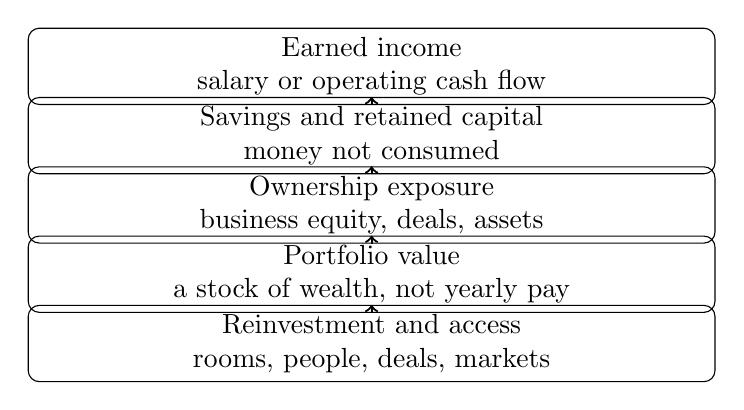
\begin{tikzpicture}[
  node distance=0.88cm,
  every node/.style={
    draw,
    rounded corners,
    align=center,
    text width=0.70\linewidth,
    minimum height=0.76cm
  },
  arrow/.style={->, thick}
]
\node (income) {Earned income\\salary or operating cash flow};
\node (saving) [below of=income] {Savings and retained capital\\money not consumed};
\node (ownership) [below of=saving] {Ownership exposure\\business equity, deals, assets};
\node (portfolio) [below of=ownership] {Portfolio value\\a stock of wealth, not yearly pay};
\node (access) [below of=portfolio] {Reinvestment and access\\rooms, people, deals, markets};
\draw[arrow] (income) -- (saving);
\draw[arrow] (saving) -- (ownership);
\draw[arrow] (ownership) -- (portfolio);
\draw[arrow] (portfolio) -- (access);
\end{tikzpicture}
\caption{A transcript-derived reconstruction of the main pathway that recurs across the Houston interviews. The diagram distinguishes income, savings, ownership, portfolio value, and access.}
\end{figure}

This is not a formula for becoming wealthy. It is a guide for reading the evidence. The first speaker begins with foundation. The second speaker moves us into ownership and portfolio value. Later speakers return us to operating discipline, sales, real estate, relationships, and product margins.

\section{Foundation Before Speed}

The first full interview slows the montage down. The speaker says that he runs a company, solves problems, and now leads an insurance brokerage firm described as a multi-billion-dollar company. His explanation is not a shortcut. It is leadership, people, education, and time inside a discipline.

Asked what he would tell himself at the beginning, he joins two ideas that should not be separated. First, be bold. Second, get a foundation. Young people, he says, often want to make it as fast as they can; his counsel is to spend four or five years understanding the discipline and then go do it yourself. The first mechanism is competence before leverage.

The interview then turns to personal finance. The speaker recommends \emph{The Wealthy Barber} and \emph{The Millionaire Next Door}, then says to save early. The transcript contains the phrase ``rule of seven,'' but the usable claim is the adjacent savings recommendation: save 10 to 20 percent.

We write annual savings as
\begin{equation}
S=sY,
\end{equation}
where \(s\) is the savings rate. The transcript-backed range is
\begin{equation}
s\in[0.10,0.20].
\end{equation}
The same exchange mentions income of roughly
\begin{equation}
Y\approx \$70{,}000 \hbox{ to } \$80{,}000.
\end{equation}
So the corresponding annual savings range is
\begin{align}
S_{\min} &=0.10(\$70{,}000)=\$7{,}000,\\
S_{\max} &=0.20(\$80{,}000)=\$16{,}000.
\end{align}

That arithmetic does not prove the speaker's claim that a saver will be a millionaire by age 30 or 40. It does something more modest and more useful: it shows the conversion from earned income into investable capital. Savings is not wealth by itself; it is the raw material from which ownership becomes possible.

\subsection{Question \& Answer}

\paragraph{Question.}
Can ordinary earned income become wealth, or does wealth require ownership leverage?

\paragraph{Answer.}
The first interview says ordinary income can begin the process if it is paired with discipline: learn a field, save early, and build a foundation. But the later interviews show why saving alone is not the whole story. Savings creates capital; ownership determines whether that capital remains small, compounds slowly, or gains exposure to much larger outcomes.

The speaker also adds a philanthropic note: he talks about helping people, giving money away, and having a 501c. In the rhythm of the interview, that matters because wealth is not presented only as accumulation. It is also presented as responsibility and usefulness after accumulation.

\section{Portfolio Value Is Not Annual Income}

The next major interview changes the scale. The speaker describes starting in oil and gas as a project manager after attending TCU and Rice University. From project management, he says he became an angel investor, had successful exits, and then started a private equity firm. The vehicle has changed: from labor income to ownership exposure.

The host asks the question from the montage: what is the most money you ever made in a single year? The answer is the key technical moment of the interview. The speaker does not answer in terms of salary. He says it is not really based on dividends or what he makes from companies; it is more about what he has as far as portfolio value. Then he gives the range: about \$420 million.

In notation, the interview claim is
\begin{equation}
P\approx \$420{,}000{,}000.
\end{equation}
But \(P\neq Y\). Portfolio value is a stock. Annual income is a flow. Dividends are a flow. Realized sale proceeds are another flow. A large portfolio may or may not produce large annual cash income, depending on liquidity, distributions, taxes, leverage, and valuation.

\subsection{Question \& Answer}

\paragraph{Question.}
When someone says he made or has ``\$420 million,'' what exactly is being measured?

\paragraph{Answer.}
In this interview, the speaker himself points away from ordinary annual income. He describes the number as portfolio range, not salary and not dividends. The notes should therefore treat \(P\approx \$420\) million as an interview claim about portfolio value. It should not be rewritten as yearly cash income.

This distinction is not pedantry. It changes the lesson. If the number is salary, then the question is how to get a very high-paying job. If the number is portfolio value, then the question is how ownership, exits, valuation, and deal access produced a large stock of wealth.

\section{Risk, Asymmetry, and Access}

The host then asks for the biggest risk. The answer is Snapchat. The speaker says Snapchat was raising a seed round in 2010 and that he invested a large amount relative to his situation as a project manager. He gives the two numbers we need: salary of \$80,000 and an investment ask of \$20,000.

The simplest useful calculation is exposure:
\begin{equation}
E=\frac{I}{Y}.
\end{equation}
With the transcript's numbers,
\begin{equation}
E=\frac{\$20{,}000}{\$80{,}000}=0.25.
\end{equation}
So the risk was not merely that \$20,000 is a large number. It was large relative to the income base: one quarter of a year's salary.

\paragraph{Worked exposure calculation.}
\begin{enumerate}
\item Start from the annual salary claim, \(Y=\$80{,}000\).
\item Start from the investment claim, \(I=\$20{,}000\).
\item Define exposure as investment divided by annual salary:
\[
E=\frac{I}{Y}.
\]
\item Substitute the transcript values:
\[
E=\frac{20{,}000}{80{,}000}=0.25.
\]
\item Interpret the result as concentrated personal exposure: the investment represented 25 percent of one year's salary.
\end{enumerate}

The speaker later claims about \$72 million from Snap and other companies in his portfolio:
\begin{equation}
V\approx \$72{,}000{,}000.
\end{equation}
Here we must be careful. The transcript does not cleanly say that \(V\) came only from the \$20,000 Snapchat investment. It says Snap and the other companies in the portfolio. A general return multiple is
\begin{equation}
M=\frac{V}{I},
\end{equation}
but in this case the clean multiple is uncertain because the outcome combines several holdings. The right lesson is asymmetry, not a verified ratio. A finite investment can be lost, while ownership in a successful company can produce an outcome far beyond the original salary scale.

The speaker then names another mechanism: marketing. Asked what takes a business from seven to eight and eventually nine figures, he answers with marketing. The host's recap turns the story into a network thesis: to find companies, deals, and rooms, the investor had to work with people who were wealthier and better connected.

That is the bridge from risk to access. Capital matters, but access determines which risks are available in the first place.

\section{Operations: Showing Up, Details, and Listening}

After the portfolio story, the episode returns to operating businesses. This is an important change in rhythm. If we only keep the angel-investment story, we miss the disciplines that make a business credible enough to attract customers, employees, lenders, or investors.

A restaurant operator gives the simplest operating principle: 90 percent of success is showing up. He explains the phrase. If you show up to work, you get work done, and people trust you. They know you will be there like clockwork. Reliability converts time into trust:
\begin{equation}
\hbox{repeated presence}
\longrightarrow
\hbox{trust}
\longrightarrow
\hbox{opportunity}.
\end{equation}
This is not a law of nature. It is the mechanism the speaker describes.

He then turns from presence to detail: remembering children's names, having birthday cakes, surprising people, writing handwritten letters, and thanking customers for coming into the restaurant. These are small actions, but the business claim is that small repeated acts of recognition become differentiation.

The Lamborghini segment follows as a motivational interlude. The advice is to put the desire into the universe, visualize it, see it, go after it, and not give up. The claim is less concrete than the operating and investment material, so the notes should not let it dominate the chapter. Its useful place is as a bridge from belief to action: aspiration becomes meaningful only when joined to persistence and decisions.

The next interview, with the port-infrastructure engineer, makes that bridge more concrete. He describes decisions as a kind of ledger: early choices compound and can cascade through life, while later choices become more valuable. He also praises being genuine while adapting to the situation, and not needing to be the biggest person in the room. The lesson is judgment under changing conditions.

Later, an industrial real estate speaker returns us to operations. He says his company buys or builds and leases large industrial properties across the country. He claims over a million dollars in a single year and says the secret to scaling is work volume:
\begin{equation}
H\approx 60\ \hbox{hours/week}.
\end{equation}
When asked about sales, he says the best way to close deals is to listen. The reason is practical: if we do not understand perspectives, needs, and wants, we cannot fulfill them. In this part of the transcript, sales is not pressure. Sales is diagnosis.

\section{Marketing, Relationships, and Brand Formation}

Marketing first appears in the private equity interview as the answer to scaling from seven to eight and eventually nine figures. It appears again in the renewable-energy social media marketer, who says the secret to marketing and building a strong brand is networking and building relationships outside social media platforms. This is a useful correction. Marketing is not merely posting; in these interviews it means distribution, reputation, and relationship density.

The same speaker claims annual income probably in the range of \$350,000 to half a million:
\begin{equation}
Y\approx \$350{,}000 \hbox{ to } \$500{,}000.
\end{equation}
She also recommends learning to save early, investing as soon as possible, and considering real estate properties and worthwhile companies. Again, the transcript gives claims and categories rather than a formal investment model.

The champagne founder closes the marketing arc. He says he set out to redefine champagne. His story runs through the restaurant industry, oil and gas, travel, wine regions, terroirs, and turning passion into a business case. His sales explanation is twofold: relationships and a product that is second to none. He contrasts that with conglomerates hiding behind large labels.

This final interview gives the most explicit product-market discipline. He advises founders to know the market, know the competitors, know the price point, know what premium positioning permits, nail the margins, and set contingencies because costs often come out higher than expected. A clean bookkeeping relation for that point is
\begin{equation}
\hbox{gross margin}
=
\frac{\hbox{price}-\hbox{unit cost}}{\hbox{price}}.
\end{equation}
The interview does not give a spreadsheet. It gives a discipline: premium positioning without margin control is fragile. If costs rise and no contingency was built in, the apparent premium business can lose its economics.

\begin{table}
\centering
\begin{tabular}{p{0.21\linewidth}p{0.23\linewidth}p{0.25\linewidth}p{0.17\linewidth}}
\hline
Context & Concrete claim & Mechanism & Caution\\
\hline
Insurance brokerage & Multi-billion-dollar company & Leadership, people, foundation & Claimed scale\\
Savings advice & Save 10--20 percent & Convert income into capital & Not a guarantee\\
Angel investing & \$20k risk on \$80k salary & Ownership asymmetry & Outcome mixed with portfolio\\
Restaurant & Show up and remember details & Trust and differentiation & Local operating claim\\
Industrial real estate & 60 hours/week and listening & Work volume and diagnosis & Not universal formula\\
Champagne & Research price, market, margins & Premium positioning & Costs may exceed plan\\
\hline
\end{tabular}
\caption{A compact separation of anecdote, claim, mechanism, and caution from the transcript.}
\end{table}

\section{Real Estate, Tax Caveats, and Asset Structure}

Real estate appears several times. One speaker works in industrial real estate, buying or building and leasing large properties. Another mentions real estate investment trusts and a \$1.2 million deal. The transcript also includes claims about tax breaks, caveats, nuances, buying assets through entities, leasing assets to oneself, and write-offs.

This material should be preserved, but cautiously. It is legally and financially sensitive, and parts of the transcript are garbled. We can still extract the conceptual distinction:
\begin{equation}
\hbox{asset return}
\neq
\hbox{tax effect}
\neq
\hbox{cash income}.
\end{equation}
A business owner may care about all three, but they are not the same number. The interview claims that structures, entities, and tax treatment can affect how wealth is preserved. These notes should not convert that into tax advice. The usable lesson is that advanced ownership requires understanding structure, not merely buying an asset.

\subsection{Question \& Answer}

\paragraph{Question.}
Are tax breaks and entity structures the wealth mechanism, or are they secondary?

\paragraph{Answer.}
In this transcript, they are secondary but important. The primary mechanisms are ownership, cash flow, deal access, operations, sales, and product-market discipline. Entity structure and tax treatment affect how gains are held, protected, or reinvested. Because this section of the transcript is partly garbled and the subject is technical, the chapter should treat these comments as prompts for professional advice, not as instructions.

\section{Summary: Wealth as Repeated Leverage}

No single interview gives the whole map. The insurance executive gives foundation, saving, leadership, and service. The investor gives ownership risk, portfolio value, marketing, and access. The restaurant owner gives showing up and details. The Lamborghini exchange contributes belief and visualization, but it becomes useful only when attached to action. The engineer gives decision quality and adaptability. Industrial real estate gives work volume and listening. Social media marketing gives relationships beyond platforms. The real estate and REIT discussion gives caution around structure. The champagne founder gives research, margins, premium positioning, relationships, product quality, and contingencies.

A compact summary of the transcript's recurring mechanisms is
\begin{align}
\hbox{wealth building}
&\approx
\hbox{discipline}
+\hbox{ownership}
+\hbox{asymmetry}
+\hbox{trust} \notag\\
&\quad
+\hbox{relationships}
+\hbox{research}
+\hbox{margin control}
+\hbox{judgment}.
\end{align}
This is not a formula that computes net worth. It is a sorting device. The interviews begin with visible outcomes, but the useful work begins when we ask what kind of number we are hearing, what risk produced it, what operating behavior sustained it, what relationships made it possible, and what cautions keep the story source-conscious.